% Created 2020-09-23 Wed 14:05
% Intended LaTeX compiler: pdflatex
\documentclass[11pt]{article}
\usepackage[utf8]{inputenc}
\usepackage[T1]{fontenc}
\usepackage{graphicx}
\usepackage{grffile}
\usepackage{longtable}
\usepackage{wrapfig}
\usepackage{rotating}
\usepackage[normalem]{ulem}
\usepackage{amsmath}
\usepackage{textcomp}
\usepackage{amssymb}
\usepackage{capt-of}
\usepackage{hyperref}
\author{adam}
\date{\today}
\title{}
\hypersetup{
 pdfauthor={adam},
 pdftitle={},
 pdfkeywords={},
 pdfsubject={},
 pdfcreator={Emacs 26.3 (Org mode 9.3.8)}, 
 pdflang={English}}
\begin{document}

\tableofcontents

\textbf{Introduction to the subject of electronic music}

\section{Overview}
\label{sec:org6ebc898}
\subsection{Course Structure}
\label{sec:org7f27f0c}
The lectures are designed as an introduction to Electronic Music,
Sound Design and Creative Programming. There are 10 dates for lectures
that  allow us to make this brief introduction. Us refers to the
teachers,  students and me the course lecturer as well as the author
of these notes.  Throughout the course, an informal and personal way
of addressing  will be used to explain specific tasks and convey
information.  This will be familiar to those who have attended
lectures at the  Vienna Music Institute as well as something new to
some  who are used to the more formal approach.

One of the key principles we will focus on over the next semester is
the  idea of ​​parametric design. And, in essence, this series of
lectures  can be described in detail as a general introduction to some
basic principles of parametric design. At lecture 5, this topic will
be  presented in detail, it will be enough for us now and in the
upcoming  lectures to get to know the individual modules such as
oscillators,  filters, amplifiers, sequencers and aspects of control. 


\subsection{Teaching Philosophy}
\label{sec:orgaa34826}
The subject can be subdivided into the following categories

\begin{itemize}
\item Project Organisation
\item Sound Design
\item Sound Synthesis
\item Digital Signal Processing (DSP)
\item Function and algorithm design
\item Parametric Control
\end{itemize}

In creating these categories, I’ve tried to represent some of the core
principles of electronic music and also to do this in a way that
allows  some access to the first principles at the root of design and composition. 

\subsection{A Symbolic Patch Language for Electronic Music}
\label{sec:org0686842}

To represent particular concepts, we‘ll be using a graphical patch
language  throughout the course. It will help to know for now some of
the basic elements, objects or modules that we will need to
represent. 

\begin{verbatim}

[osc]        <amp>        |\env/|        *filt*        °°seq°°        

dac|>        |<adc

\end{verbatim}


It might help to think about a patch as a kind of instrument, and these modules as the individual parts of that instrument. Surprisingly, it‘s not always immediately obvious to everyone that a guitar is created by setting together a number of parts like: strings, body, neck, fretboard, bridge, etc. The manner of construction has been informed by the physical principles of acoustics and also the practical necessities of musicians. In this course it will be of huge advantage to you to understand some basic things about acoustics and your own practical needs as a musician. Of course, we won‘t be making guitars, but as I already mentioned, it helps to think about creating electronic music in terms of putting together instruments and using them to create music. 

\subsection{Portability}
\label{sec:org3961620}
The aim of the lectures is to learn the basics of electronic music. In this sense, we focus primarily on the principles and techniques that apply to the creation of electronic music, and secondarily on the learning of paradigm-specific methods.
In any case, basic principles can best be illustrated by practical examples. Sometimes it's easier for me to introduce certain concepts in the classroom with proprietary software. In such cases, the goal should not be to spend all your money on acquiring copies of the software you are using, but to find out how the techniques described can be practiced with freely available software. In the first place, you should use two programs in combination to work through the examples that appear in each lesson and work as homework assignments: VCV Rack and Reaper. 

\subsection{Reading Material}
\label{sec:org2387a46}

A very good resource if you want to brush up on some of the basics of the types of mathematics that are found at the root of musical systems
\begin{itemize}
\item Gareth Loy, \textbf{Musimathics vol. I-II}, MIT Press
\end{itemize}

Great reference for many of the essential topics of computer music
\begin{itemize}
\item Curtis Roads: \textbf{The Computer Music Tutorial}, MIT Press
\end{itemize}

Very well written book on modular synthesis, with lots of worthwhile exercises that will form the basis of our practical work throughout the course
\begin{itemize}
\item Allan Strange: \textbf{Electronic Music Systems Techniques and Controls}, Wm-C Brown Company Publishers, 1972
\end{itemize}

\section{Audio Synthesis}
\label{sec:org47a512c}
\subsection{Oscillators and Waveforms}
\label{sec:orgde758bb}
Typically an oscillator will be at the root of a synthesis patch. 
In order to hear a specific pitch, one can set the oscillator to 
generate a voltage at the desired frequency.  
Note that there is also a relationship between pitch and perceived 
loudness: a tone played at 1024Hz will sound louder than a tone played with the same gain at 64 Hz.

\subsubsection{Sine Waves and the Harmonic Series}
\label{sec:org4d46036}
Come to think of it, this could be a good time to mention the harmonic
series, we'll come back to the relationship between pitch and loudness
in a minute. 

\begin{center}
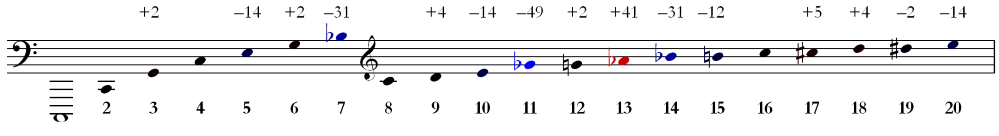
\includegraphics[width=.9\linewidth]{./images/Harmonic_Series1.png}
\end{center}

In the world of synthesizers and especially electronic music, an
oscillator will typically be looking for a precise definition of pitch
in order to produce a tone. 

\begin{center}
\begin{tabular}{lrr}
Pitch name & partial num. & Frequency (Hz)\\
\hline
c, & 1 & 64\\
c & 2 & 128\\
g & 3 & 192\\
c' & 4 & 256\\
e' & 5 & 320\\
g' & 6 & 384\\
bf' & 7 & 448\\
c'' & 8 & 512\\
d'' & 9 & 576\\
e'' & 10 & 640\\
gf'' & 11 & 704\\
g'' & 12 & 768\\
af'' & 13 & 832\\
bf'' & 14 & 896\\
b'' & 15 & 960\\
c''' & 16 & 1024\\
\end{tabular}
\end{center}


\subsection{A side note on midi to herz conversion}
\label{sec:org816d9e2}
Practically speaking, you will rarely have to think about doing these
types of conversions from a specific pitch to a midi number. Midi is a
really useful protocol that maps an equal tempered tuning system to
integer values in the range of (0-127).


\section{Exploring harmonics: \url{https://teropa.info/harmonics-explorer/}}
\label{sec:org9d45ec8}

\subsection{Waveform Types}
\label{sec:orgd814e18}
Of course, a spectrum analysis of the tone produced by a musical
instrument would reveal the presence of individual frequency
components. These are basically packets of energy focused around
certain points in time. Pythagaros or Plato or one of those fellows
would have probably started waxing lyrical about the harmony of the
spheres at this point. 
The main point here is that you don't need to think too deeply about
the concept of \emph{spectrum analysis} for now, maybe think about it as a
type of sonic x-ray that can reveal some interesting truths about the
nature of a sound. 
The whole point of mentioning analysis at all is that it can be quite
useful when used in combination with synthesis. If fact the practice
of the \emph{analytic-synthetic} method also goes all the way back to the
greeks. But that's getting slightly off-topic.   

To summarize about waveforms: depending on how they are combined,
simple sine-wave components can create more complex wavetypes. The
tones produced by musical instruments sound themselves complex and can
be analyzed to reveal the underlying structure. There are a few main
types of waveform that are typically found as settings on an oscillator.

\begin{center}
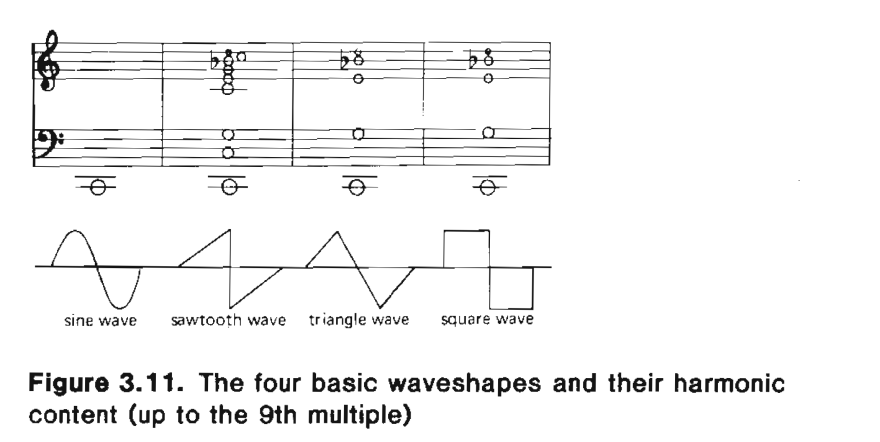
\includegraphics[width=.9\linewidth]{./images/waveforms.png}
\end{center}

\subsection{Oscillator Controls}
\label{sec:org2d4b8ca}
\subsubsection{Tuning}
\label{sec:orgd8ad21d}
\begin{itemize}
\item Offset
\item Finetune
\end{itemize}

\subsubsection{Pitch input}
\label{sec:org0a389cf}
\begin{itemize}
\item Midi
\item Control Voltage
\end{itemize}

\subsubsection{Frequency Modulation (FM)}
\label{sec:org76dbeba}
We'll go into some more detail about frequency modulation (and
modulation in general) later on in the course. It just might be
useuful to point out that most oscillators will typically have a
control for FM.

\subsubsection{Pulse width}
\label{sec:orgdaf8041}
On the square wave setting, it is possible to control the length of
the \emph{duty cycle} of a square wave. Basically, if we were using the
oscillator to open some sort of a gate, the gate would remain open for
the length of time that the square wave is non-zero. 

\begin{verbatim}
      _____       _____       _____
     |     |     |     |     |     |
     |     |     |     |     |     |
_____|     |_____|     |_____|     |_____
      ___         ___         ___
     |   |       |   |       |   |
     |   |       |   |       |   |
_____|   |_______|   |_______|   |________
      _           _           _
     | |         | |         | |
     | |         | |         | |
_____| |_________| |_________| |__________

\end{verbatim}

\subsection{Additive Synthesis}
\label{sec:org462176f}
Very simply put, additive synthesis is the idea of building up complex
sounds from very, very simply components. Most typically these are sin
tones. The link above connects to an interesting application written
in javascript. It's possible to see how the combination of different
sets of partials can produce specific waveshapes. 

\subsubsection{Building a hammond organ}
\label{sec:orgc2d97da}
This series of videos describes how to build a hammond organ style
synthesizer using vcv rack: \url{https://youtu.be/kZJF50joo2w}



\subsection{Subtractive Synthesis}
\label{sec:org74fa51c}
\subsubsection{Sawtooth and Other Complex Waveforms}
\label{sec:org6ac50c6}
\subsubsection{Filters}
\label{sec:org5a1c2fb}

\subsection{Envelopes}
\label{sec:orge0efa47}


\section{Musical Signals}
\label{sec:org72c67a0}
\subsection{Sequencers}
\label{sec:orgfa76215}
\subsubsection{Modular Style}
\label{sec:orga83c732}
\subsubsection{DAW Style}
\label{sec:org7319f46}
\subsection{Quantization}
\label{sec:orgc100e17}
\subsubsection{Pitch Quantization}
\label{sec:org0316514}
\subsubsection{Offsets}
\label{sec:orgd01df69}
\subsubsection{Harmonization}
\label{sec:org829b5a2}
\subsection{Midi}
\label{sec:org4918a72}
\subsubsection{Rhythmic Quantization}
\label{sec:org6cb4663}

\section{Modulation}
\label{sec:orgb763e4f}
\subsection{Sub-Audio Rate Modulation}
\label{sec:org152b0f2}
\subsubsection{Definition}
\label{sec:orgad81fc9}
\subsubsection{Frequency Modulation (FM)}
\label{sec:org4e7fe77}
\subsubsection{Amplitude Modulation (AM)}
\label{sec:orgdddca22}
\subsection{Audio Rate Modulation}
\label{sec:org0b31587}
\subsubsection{Sidebands and Timbre}
\label{sec:orga8ed470}
\subsubsection{FM}
\label{sec:orgd70b1da}
\subsubsection{AM}
\label{sec:orgfc0e124}

\section{Parametric Design}
\label{sec:org0bb6ae8}
\subsection{A grammar for electronic music}
\label{sec:orgb031530}

\section{DSP}
\label{sec:org05dd794}
\subsection{Sampling}
\label{sec:orgfb83e5c}
\subsection{Effects}
\label{sec:orgb086068}
\subsubsection{Delay}
\label{sec:org6f6d58c}
\subsubsection{Reverb}
\label{sec:orgbdb2a30}

\section{Advanced Synthesis Techniques}
\label{sec:orgb1936f6}
\subsection{Physical Modelling}
\label{sec:orgd13b5f3}

\section{Project work}
\label{sec:org98e0629}
\subsection{in a DAW}
\label{sec:org43e83d5}
\subsection{Voice Assignment}
\label{sec:orga7faff1}

\subsection{Appendix A}
\label{sec:org23c8300}
\subsubsection{Program selection, installation and directory structure}
\label{sec:org5a8e7d2}
\subsubsection{Project organisation in Digital Audio Workstations}
\label{sec:org8df52e7}
\end{document}
